\section*{Part 2}
\subsection*{2.1}
\begin{multicols*}{2}
\subsubsection*{Evaluation function}
Our evaluation function is
\begin{equation}
  blue_{score} - green_{score}
\end{equation}
where the $blue_{score}$ is the blue player's score for a node at which the depth limit is reached and $gree_{score}$ is that for the green player. This evaluation function assumes the players' current scores up to this point are representative of the players' competitiveness throughout the rest of the game; at worst, we assume that the players are equally competitive from this node onwards and will split the remaining available points equally.

In the case where the players' current scores are representative of their relative level competitiveness/competency against the other, it would make sense to pick the node that maximizes the difference between the green player's score and that of his opponent, which would allow the green player to win by a larger margin and buffer any potential loss in case the blue player forces him into a less favorable situation.

In the case where the players are equally competitive, we would also like to pick the node with the largest difference in scores. Since we assume the players will be equally matched from this point on, 

\subsubsection*{Results}
\paragraph*{Minimmax vs. minimax}
Below are our results. Read down the left column, then down the right.

The total scores for each player can be seen within the figures. The total and average numbers of nodes expanded by each AI player, and the average time to make a move are shown in a table below each figure.

\begin{figure}[H]
\centering
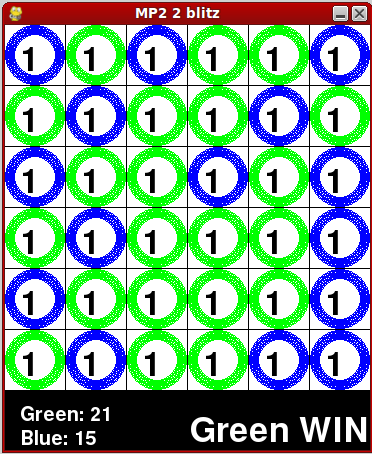
\includegraphics[width=0.3\textwidth]{graphics/mm_keren.png}
\caption{Keren}
\end{figure}
\begin{tabular}{l|r|r|r}
  Player & total \# nodes & avg \# nodes & avg time \\
  \hline
  Blue & 217740 & 12096.6666667 & 2.92898527781 \\
  Green & 194736 & 10818.6666667 & 2.62170659171 \\
\end{tabular}

\begin{figure}[H]
\centering
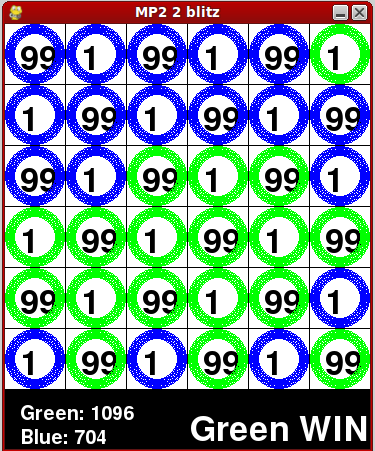
\includegraphics[width=0.3\textwidth]{graphics/mm_narvik.png}
\caption{Narvik}
\end{figure}
\begin{tabular}{l|r|r|r}
  Player & total \# nodes & avg \# nodes & avg time \\
  \hline
  Blue & 217740 & 12096.6666667 & 2.92898527781 \\
  Green & 194736 & 10818.6666667 & 2.62170659171 \\
\end{tabular}

\begin{figure}[H]
\centering
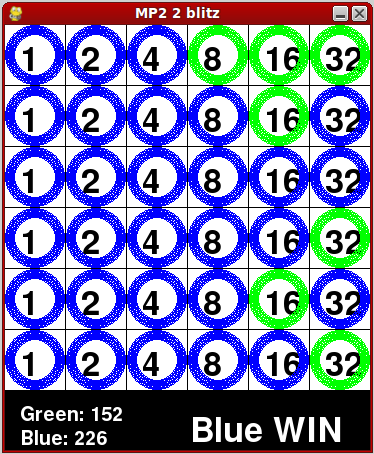
\includegraphics[width=0.3\textwidth]{graphics/mm_sevastopol.png}
\caption{Sevastopol}
\end{figure}
\begin{tabular}{l|r|r|r}
  Player & total \# nodes & avg \# nodes & avg time \\
  \hline
  Blue & 217740 & 12096.6666667 & 2.97655142678 \\
  Green & 194736 & 10818.6666667 & 2.67341685295 \\
\end{tabular}

\begin{figure}[H]
\centering
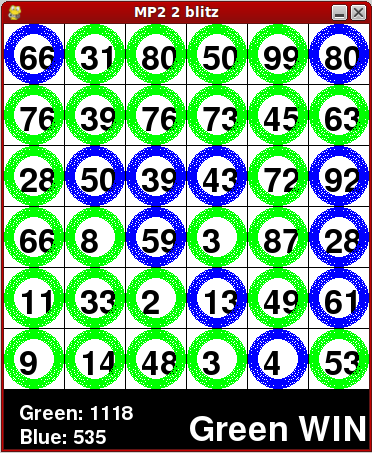
\includegraphics[width=0.3\textwidth]{graphics/mm_smolensk.png}
\caption{Smolensk}
\end{figure}
\begin{tabular}{l|r|r|r}
  Player & total \# nodes & avg \# nodes & avg time \\
  \hline
  Blue & 217740 & 12096.6666667 & 3.08422014448 \\
  Green & 194736 & 10818.6666667 & 2.75713196066 \\
\end{tabular}

\begin{figure}[H]
\centering
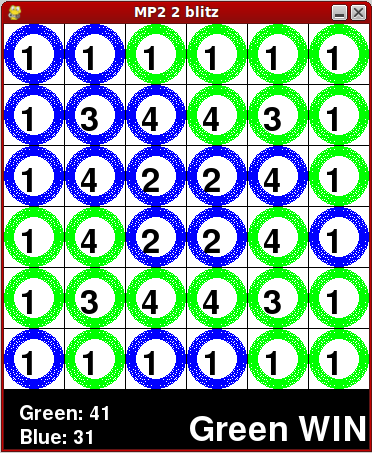
\includegraphics[width=0.3\textwidth]{graphics/mm_westerplatte.png}
\caption{Westerplatte}
\end{figure}
\begin{tabular}{l|r|r|r}
  Player & total \# nodes & avg \# nodes & avg time \\
  \hline
  Blue & 217740 & 12096.6666667 & 2.91952784856 \\
  Green & 194736 & 10818.6666667 & 2.61617973116 \\
\end{tabular}

\columnbreak
\paragraph*{Minimax vs. alpha-beta}
\mbox{}\\
\begin{figure}[H]
\centering
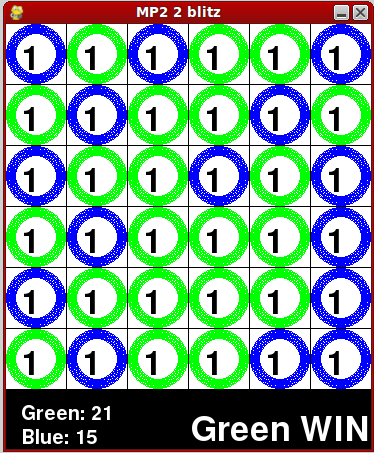
\includegraphics[width=0.3\textwidth]{graphics/ma_keren.png}
\caption{Keren}
\end{figure}
\begin{tabular}{l|r|r|r}
  Player & total \# nodes & avg \# nodes & avg time \\
  \hline
  Blue & 217740 & 12096.6666667 & 2.90004497104 \\
  Green & 9527 & 529.277777778 & 0.127783245511 \\
\end{tabular}

\begin{figure}[H]
\centering
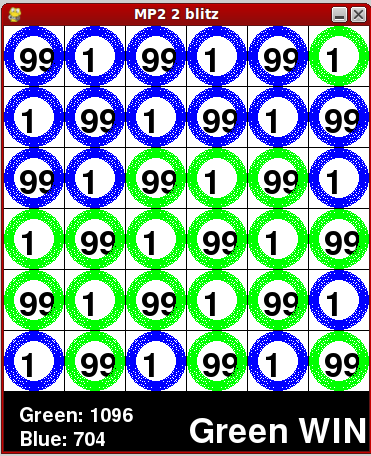
\includegraphics[width=0.3\textwidth]{graphics/ma_narvik.png}
\caption{Narvik}
\end{figure}
\begin{tabular}{l|r|r|r}
  Player & total \# nodes & avg \# nodes & avg time \\
  \hline
  Blue & 217740 & 12096.6666667 & 2.91591848267 \\
  Green & 18893 & 1049.61111111 & 0.250732925203 \\
\end{tabular}

\begin{figure}[H]
\centering
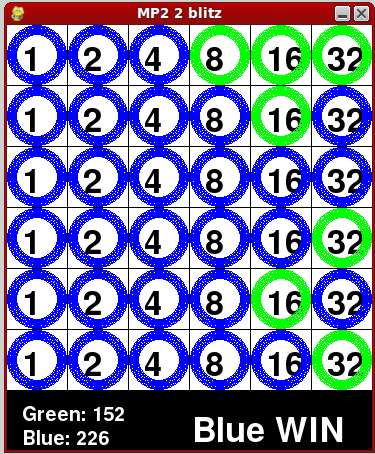
\includegraphics[width=0.3\textwidth]{graphics/ma_sevastopol.png}
\caption{Sevastopol}
\end{figure}
\begin{tabular}{l|r|r|r}
  Player & total \# nodes & avg \# nodes & avg time \\
  \hline
  Blue & 217740 & 12096.6666667 & 2.91023706065 \\
  Green & 152377 & 8465.38888889 & 2.03938767645 \\
\end{tabular}

\begin{figure}[H]
\centering
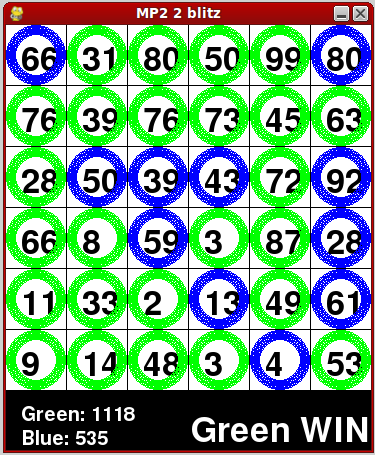
\includegraphics[width=0.3\textwidth]{graphics/ma_smolensk.png}
\caption{Smolensk}
\end{figure}
\begin{tabular}{l|r|r|r}
  Player & total \# nodes & avg \# nodes & avg time \\
  \hline
  Blue & 217740 & 12096.6666667 & 3.04809761047 \\
  Green & 76030 & 4223.88888889 & 1.07544849979 \\
\end{tabular}

\begin{figure}[H]
\centering
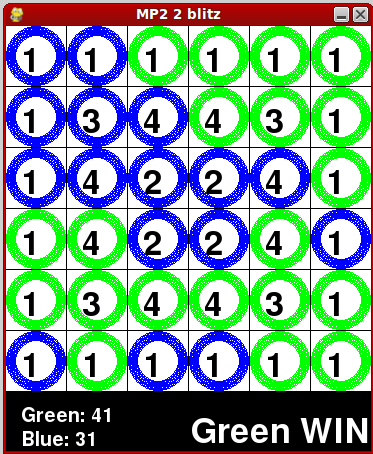
\includegraphics[width=0.3\textwidth]{graphics/ma_westerplatte.png}
\caption{Westerplatte}
\end{figure}
\begin{tabular}{l|r|r|r}
  Player & total \# nodes & avg \# nodes & avg time \\
  \hline
  Blue & 
\end{tabular}

\paragraph*{Alpha-beta vs. alpha-beta}
\mbox{}\\
\begin{figure}[H]
\centering
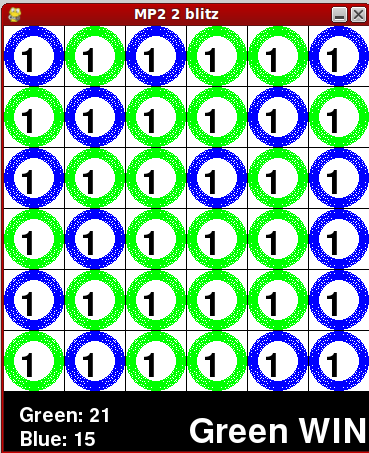
\includegraphics[width=0.3\textwidth]{graphics/aa_keren.png}
\caption{Keren}
\end{figure}
\begin{tabular}{l|r|r|r}
  Player & total \# nodes & avg \# nodes & avg time \\
  \hline
  Blue & 10483 & 582.388888889 & 0.144407219357 \\
  Green & 9527 & 529.277777778 & 0.132013400396 \\
\end{tabular}

\begin{figure}[H]
\centering
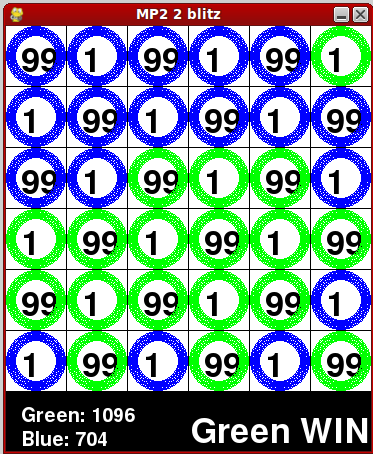
\includegraphics[width=0.3\textwidth]{graphics/aa_narvik.png}
\caption{Narvik}
\end{figure}
\begin{tabular}{l|r|r|r}
  Player & total \# nodes & avg \# nodes & avg time \\
  \hline
  Blue & 18012 & 1000.66666667 & 0.24585489432 \\
  Green & 18893 & 1049.61111111 & 0.259964439604 \\
\end{tabular}

\begin{figure}[H]
\centering
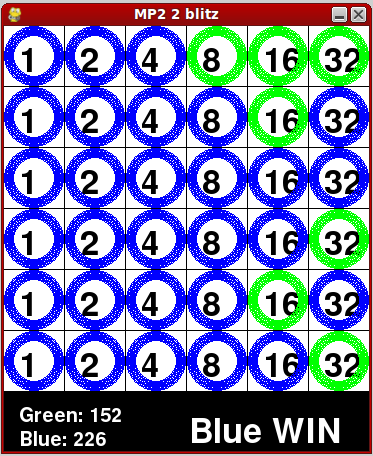
\includegraphics[width=0.3\textwidth]{graphics/aa_sevastopol.png}
\caption{Sevastopol}
\end{figure}
\begin{tabular}{l|r|r|r}
  Player & total \# nodes & avg \# nodes & avg time \\
  \hline
  Blue & 175974 & 9776.33333333 & 2.32421615389 \\
  Green & 152377 & 8465.38888889 & 2.01822400093 \\
\end{tabular}

\begin{figure}[H]
\centering
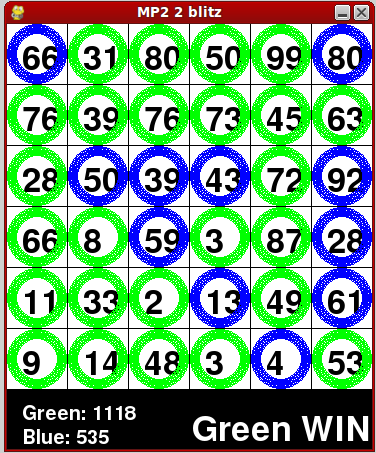
\includegraphics[width=0.3\textwidth]{graphics/aa_smolensk.png}
\caption{Smolensk}
\end{figure}
\begin{tabular}{l|r|r|r}
  Player & total \# nodes & avg \# nodes & avg time \\
  \hline
  Blue & 100949 & 5608.27777778 & 1.45887796084 \\
  Green & 76030 & 4223.88888889 & 1.1003742218 \\
\end{tabular}

\begin{figure}[H]
\centering
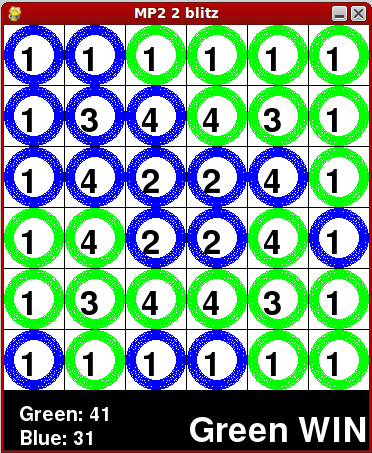
\includegraphics[width=0.3\textwidth]{graphics/aa_westerplatte.png}
\caption{Westerplatte}
\end{figure}
\begin{tabular}{l|r|r|r}
  Player & total \# nodes & avg \# nodes & avg time \\
  \hline
  Blue & 36003 & 2000.16666667 & 0.495845940378 \\
  Green & 35006 & 1944.77777778 & 0.479608231121 \\
\end{tabular}

\paragraph*{Alpha-beta vs. minimax}
\mbox{}\\
\begin{figure}[H]
\centering
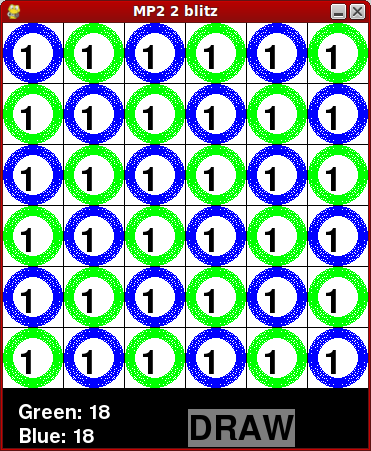
\includegraphics[width=0.3\textwidth]{graphics/am_keren.png}
\caption{Keren}
\end{figure}
\begin{tabular}{l|r|r|r}
  Player & total \# nodes & avg \# nodes & avg time \\
  \hline
  Blue & 18012 & 94 & 0.5085 \\
  Green & 9527 & 529.277777778 & 0.127783245511 \\
\end{tabular}

\begin{figure}[H]
\centering
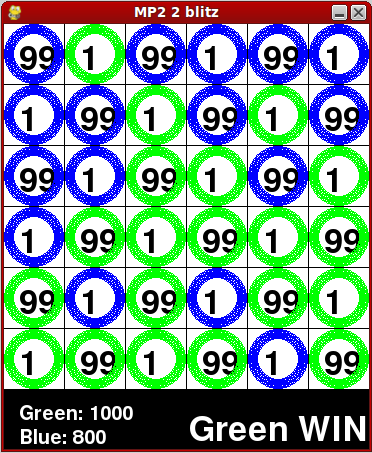
\includegraphics[width=0.3\textwidth]{graphics/am_narvik.png}
\caption{Narvik}
\end{figure}
\begin{tabular}{l|r|r|r}
  Player & total \# nodes & avg \# nodes & avg time \\
  \hline
  Blue & 18893 & 1049.61111111 & 0.250732925203 \\
  Green & 1695 & 94.1666666667 & 0.023103872935 \\
\end{tabular}

\begin{figure}[H]
\centering
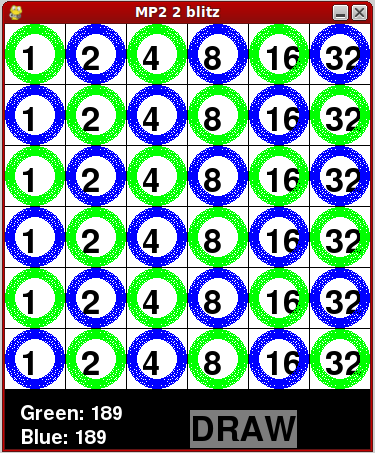
\includegraphics[width=0.3\textwidth]{graphics/am_sevastopol.png}
\caption{Sevastopol}
\end{figure}
\begin{tabular}{l|r|r|r}
  Player & total \# nodes & avg \# nodes & avg time \\
  \hline
  Blue & 7044 & 391.333333333 & 0.0933979087406 \\
  Green & 217740 & 12096.6666667 & 2.91023706065 \\
\end{tabular}

\begin{figure}[H]
\centering
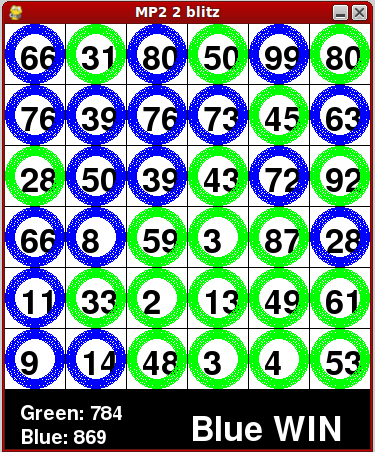
\includegraphics[width=0.3\textwidth]{graphics/am_smolensk.png}
\caption{Smolensk}
\end{figure}
\begin{tabular}{l|r|r|r}
  Player & total \# nodes & avg \# nodes & avg time \\
  \hline
  Blue & 2808 & 156.0 & 0.0399910211563 \\
  Green & 217740 & 12096.6666667 & 3.04809761047 \\
\end{tabular}

\begin{figure}[H]
\centering
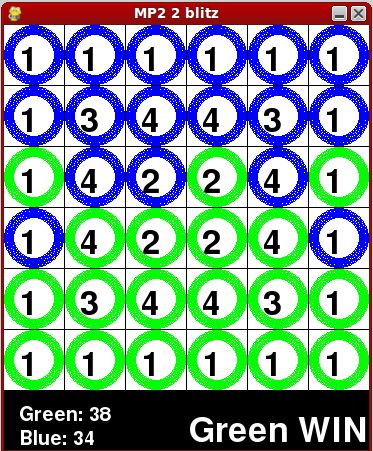
\includegraphics[width=0.3\textwidth]{graphics/am_westerplatte.png}
\caption{Westerplatte}
\end{figure}
\begin{tabular}{l|r|r|r}
  Player & total \# nodes & avg \# nodes & avg time \\
  \hline
  Blue & 2634 & 146.333333333 & 0.0353087849087 \\
  Green & 217740 & 12096.6666667 & 2.91757289569 \\
\end{tabular}

\end{multicols*}


\subsubsection*{Bonus points}
\paragraph{1.}
As seen above, we implemented a GUI to visualize the AI gameplay. It is also possible to play against the AI as either blue or green, or have two humans play as blue and green. A video of Mingyo playing against as blue against an AI using alpha-beta with depth-limit 3, 4 can be found here: https://youtu.be/pOYsBjNLKUg https://www.youtube.com/watch?v=63frlcAnE5I\&feature=youtu.be. The only rules used are from 2.1.
\paragraph{2.}
We tried expanding the Smolensk board into a 7x7 board. Shown below are the results for minimax vs minimax without the extended rules from 2.2, and the same for alpha-beta vs alpha-beta. We see that the number of nodes that both minimax and alpha-beta expand is an order of magnitude greater than for the 6x6 board.

\begin{figure}[H]
\centering
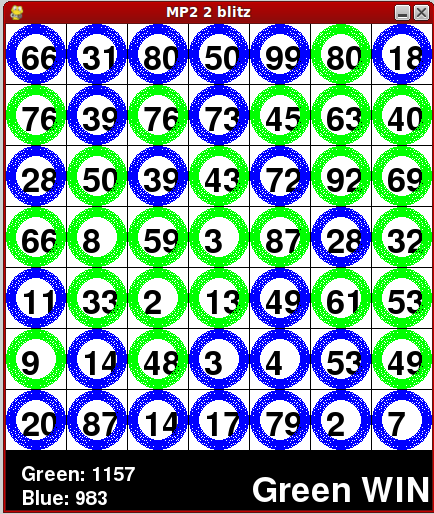
\includegraphics[width=0.3\textwidth]{graphics/mm_bigger_7x7.png}
\caption{Minimax vs minimax}
\end{figure}
\begin{tabular}{l|r|r|r}
  Player & total \# nodes & avg \# nodes & avg time \\
  \hline
  Blue & 19600 & 1088.88888889 & 0.277746717135 \\
  Green & 20825 & 1156.94444444 & 0.295267422994 \\
\end{tabular}

\begin{figure}[H]
\centering
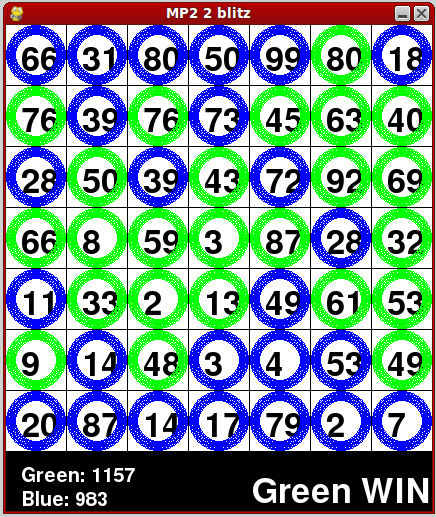
\includegraphics[width=0.3\textwidth]{graphics/aa_bigger_7x7.png}
\caption{Alpha-beta vs alpha-beta}
\end{figure}
\begin{tabular}{l|r|r|r}
  Player & total \# nodes & avg \# nodes & avg time \\
  \hline
  Blue & 4824 & 268.0 & 0.0693453450998 \\
  Green & 5272 & 292.888888889 & 0.0756442646186 \\
\end{tabular}

\paragraph{3.}
We use sorting of the child nodes to improve the efficiency of alpha-beta pruning. In alpha-beta pruning, the best thing is that you can find the minimum value among all child nodes of a min node, and the maximum value among all child nodes of a max node. If we can determine the alpha and beta value as soon as possible, we can avoid a lot of useless searching. So we use a tuple to storing the utility of child nodes along the node itself. Depends on whether its alpha or beta, we sort the child node either ascending or descending.\\
According to our experiment, running the Smolensk board with our improved algorithm is 20\% faster than the original algorithm without sorting. (Reduced from approximately 53 seconds to 39 seconds) 
\paragraph{4.}
For the flip coin part, we convert the non-deterministic problem into a deterministic problem with a fixed probability when we do our minimax/alpha-beta pruning. When calculating the utility, the utility brought by the blitz will be devided by two then added to the sum utility. When make the actual move, if the condition of blitz is satisfied, we use a random generator to determine if it can do the blitz or not, each with the possibility of 50\%.
Following is the video of flip coin game with Smolensk board with alpha-beta pruning with the depth 3.
\subsection*{2.2}
We chose to demonstrate each of the extended rules on the Smolensk board since it is most general, being the most random-looking board.
\subsubsection*{Battle}
\begin{figure}[H]
\centering
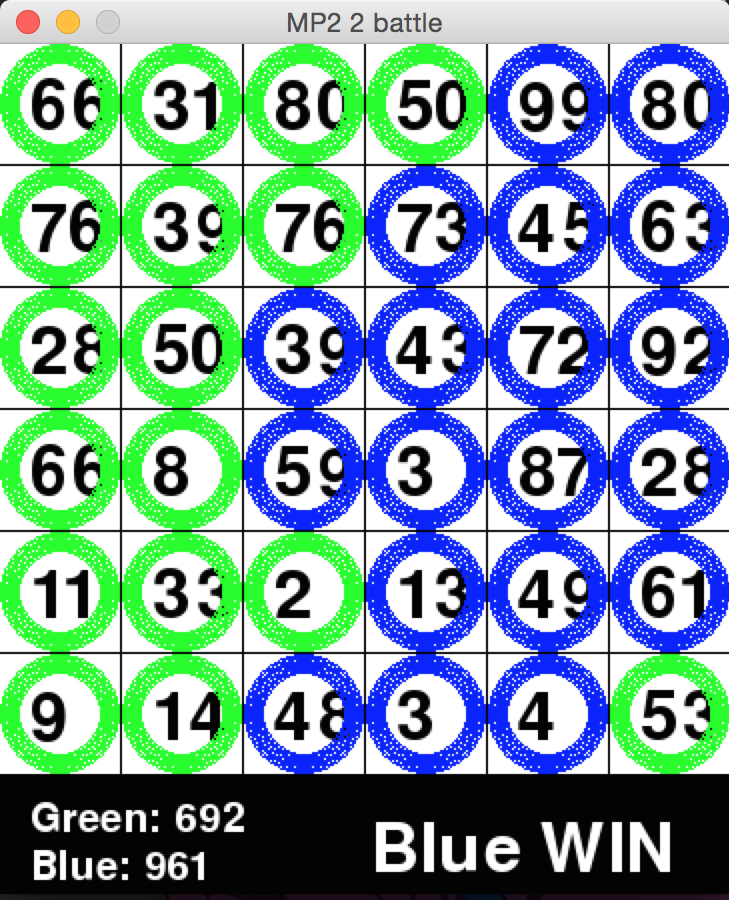
\includegraphics[width=0.3\textwidth]{graphics/battle_smolensk2.png}
\caption{Battle: Smolensk}
\end{figure}
\begin{tabular}{l|r|r|r}
  Player & total \# nodes & avg \# nodes & avg time \\
  \hline
  Blue & 43430 & 2412.77777778 & 0.847281376521 \\
  Green & 28661 & 1592.27777778 & 1.29140785005 \\
\end{tabular}

\subsubsection*{Duel}
\begin{figure}[H]
\centering
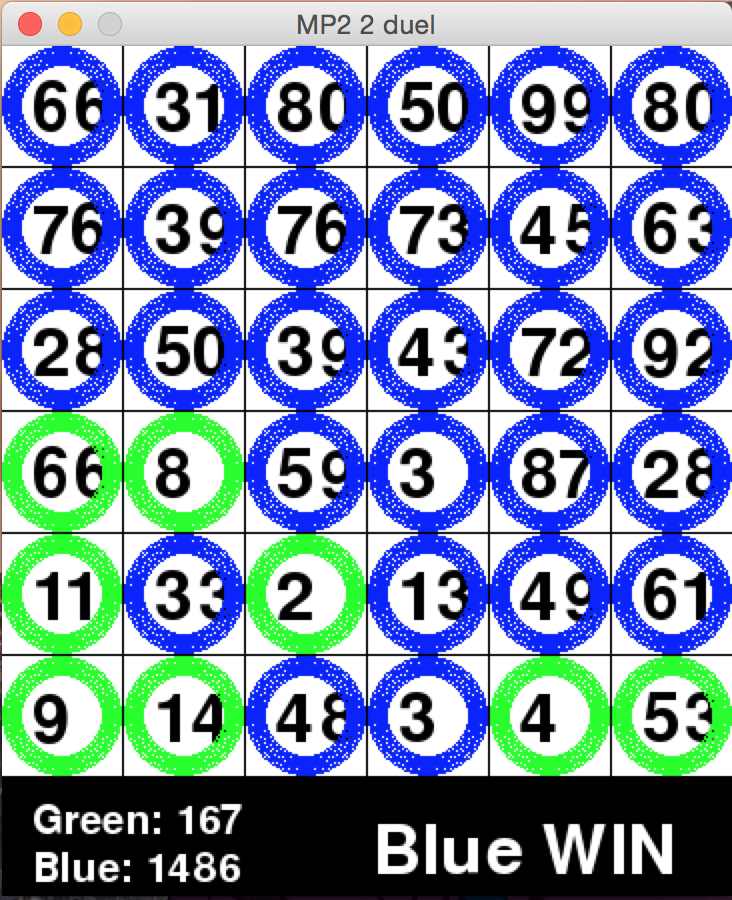
\includegraphics[width=0.3\textwidth]{graphics/duel_smolensk2.png}
\caption{Duel: Smolensk}
\end{figure}
\begin{tabular}{l|r|r|r}
  Player & total \# nodes & avg \# nodes & avg time \\
  \hline
  Blue & 23043 & 1280.16666667 & 0.785324202644 \\
  Green & 26730 & 1485.0 & 0.678644127316 \\
\end{tabular}

\subsubsection*{Attrition}
\begin{figure}[H]
\centering
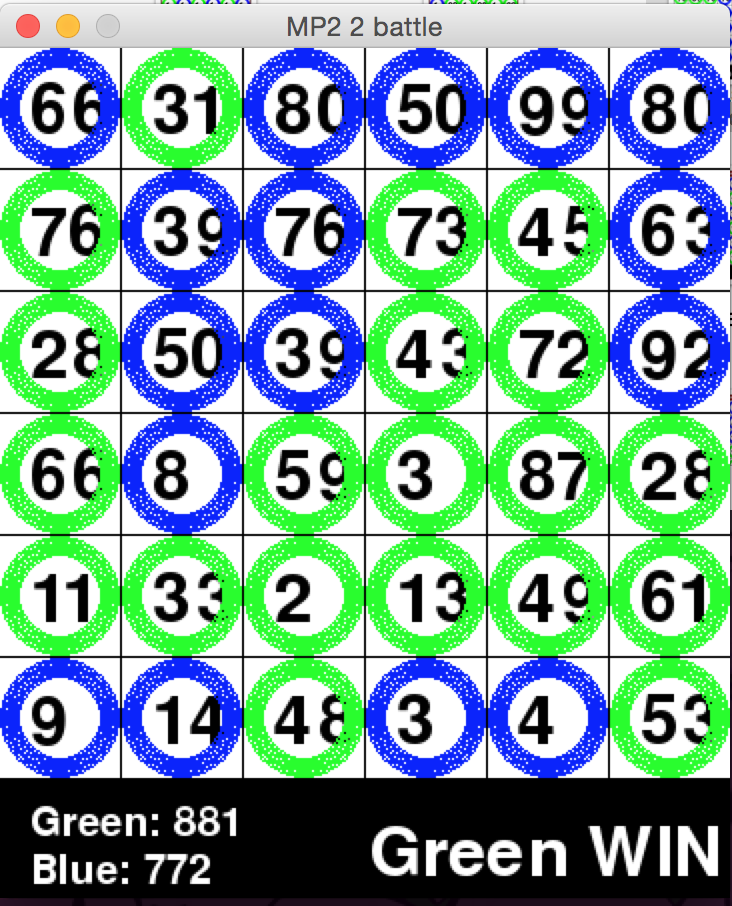
\includegraphics[width=0.3\textwidth]{graphics/attrition_smolensk2.png}
\caption{Attrition: Smolensk}
\end{figure}
\begin{tabular}{l|r|r|r}
  Player & total \# nodes & avg \# nodes & avg time \\
  \hline
  Blue & 48209 & 2678.27777778 & 1.46923801634 \\
  Green & 47628 & 2646.0 & 1.46924369865 \\
\end{tabular}

Comparing across the Smolensk board alpha-beta vs alpha-beta results for the original rules (we'll call this ``Blitz''), Battle, Duel, and Attrition, it appears that Blitz and Battle yield more linear clustering, while the remaining two rule sets yield more rectangular regions of occupation. The results for Blitz show the most scattering of units.
\iffalse
-382
Blue's node: 665
294
Green's node: 609
-385
Blue's node: 542
219
Green's node: 464
-396
Blue's node: 503
191
Green's node: 419
-399
Blue's node: 457
201
Green's node: 332
-266
Blue's node: 349
154
Green's node: 240
-454
Blue's node: 366
218
Green's node: 357
-260
Blue's node: 295
210
Green's node: 194
-117
Blue's node: 226
370
Green's node: 232
-83
Blue's node: 169
267
Green's node: 182
-269
Blue's node: 191
36
Green's node: 149
-499
Blue's node: 196
23
Green's node: 145
-335
Blue's node: 135
-185
Green's node: 95
-422
Blue's node: 95
-154
Green's node: 69
-429
Blue's node: 56
-316
Green's node: 44
-408
Blue's node: 43
-302
Green's node: 32
-390
Blue's node: 30
-374
Green's node: 19
-415
Blue's node: 16
-415
Green's node: 7
-415
Blue's node: 4
-415
Green's node: 1
game over
Avergae of blue's node: 241.0
Avergae of gree's node: 199.444444444
Expanded blue's node: 4338.0
Expanded green's node: 3590.0
green move time: 4.08695367972
blue move time: 5.11339668433

\fi
